%\documentclass[10pt, letterpaper, titlepage]{article}
\usepackage{graphicx}
\usepackage{enumerate}
\begin{document}


\textbf{Introduction}\\
It is important to study what people did and create our study on top of it. In this section, we focus on summarize previous studies of spam/ham e-mail filtering and their machine learning methods. At the end of this section, we point out the new methods and new data we use in this project to show our understanding.  \\

\textbf{Previous Studies}\\
People already came up with the idea of spam/ham e-mail filtering before 2004. In the paper \textit{Machine Learning Techniques in Spam Filtering} written by Konstantin in 2004, the experiment used four main methods : Naive Bayes, K-NN, Perceptron, and SVM. And compare accuracy rate of each methods. In this basic practice, they found the Perceptron method has the highest accuracy rate, 98.5\% with a corpus of 1099 messages. \\

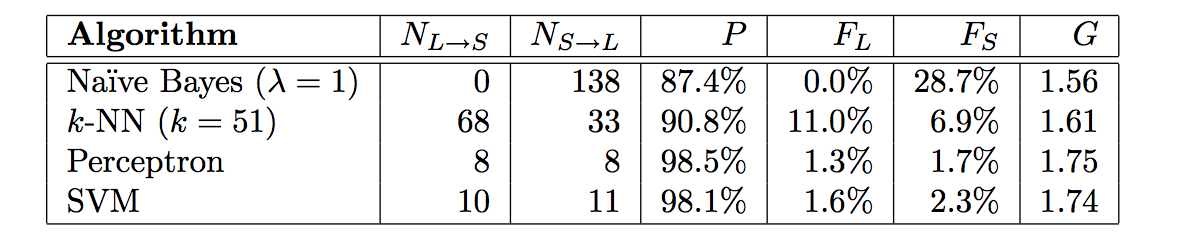
\includegraphics[scale=1.0, width=\linewidth]{2004.png}\\

In 2010, \textit{Email Spam Filtering using Supervised Machine Learning Techniques } written by V.Christina, they used Naive Bayes, J-48(Decision Tree) and Multilayer Perceptron. And they found out MLP performed the best with 99.3\% accuracy rate when experimenting with a corpus of 1500 messages.\\

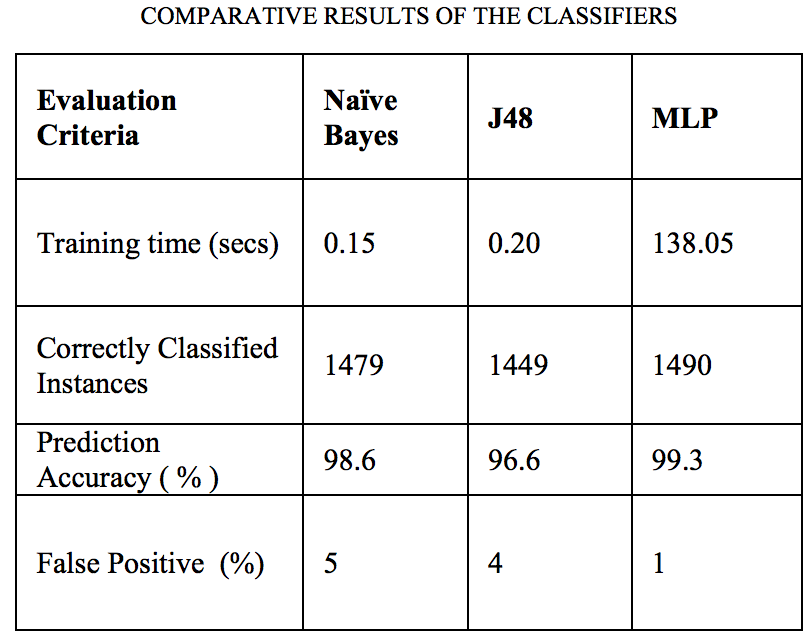
\includegraphics[width=5.5cm,height=5cm,keepaspectratio]{2010-1.png}
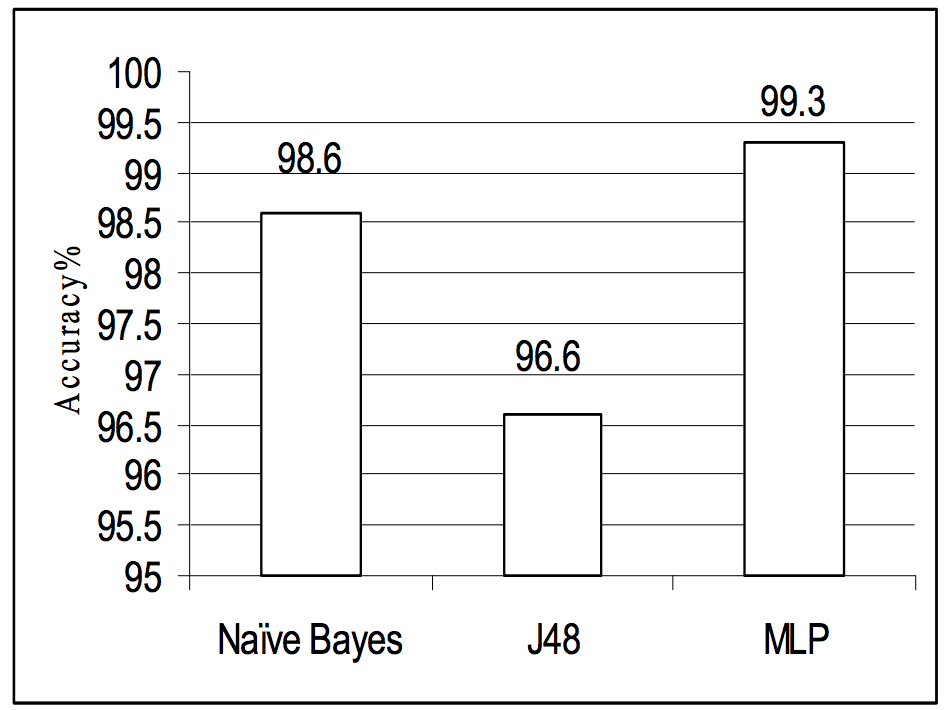
\includegraphics[width=5.5cm,height=5cm,keepaspectratio]{2010-2.png}

In 2016, \textit{Spam Mail Detection using Classification} written by Parhat and Gambhir used Naive Bayes, SVM and J-48(Decision Tree). And they found out Naive Bayes performed the best with 76\% accuracy rate in their experiment. \\ And \textit{Email Spam Detection} written by Ge and  Lauren, used the corpus from TREC 2007 with 1000 messages. They tried logistic regression, Naive Bayesian, Decision Tree and K-NN. The finally found KNN with highest 99\% accuracy rate. \\
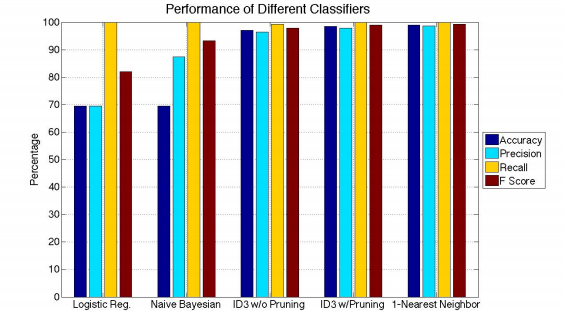
\includegraphics[width=10cm,height=5cm,keepaspectratio]{2016.png}


\textbf{Our works}\\

\begin{enumerate}
	\item \textbf{Use multiple data source}: In each paper, they mainly use a single year of corpus data. In our project, we tried to source different e-mail and integrate them. The format of each data source is different thus hard to clean. And we successfully got to manage a huge data set. 
	\item \textbf{Try 6 methods at the same time}: Previous studies compare accuracy rate with different methods, but they didn't compare them all at a time. So we studied the methods from 2004 to 2016, and apply all of possible methods with adequate tuning parameters to compare them 
	\item \textbf{Apply 1-Gram and 2-Gram}: Each paper marked that data processing step is important to a good result. Here, we introduced bag of words of 1-Gram and 2-Gram methods in the feature engineering part. And we can see different result of accuracy rate in the following section.
\end{enumerate}

%\end{document}